%\documentclass[10pt]{beamer}  % pause will take effect
\documentclass[10pt, handout]{beamer} % good for printing
\mode<presentation> {
  %\usetheme{default}
  %\usetheme{bergen}     % leftbar menu
  \usetheme[secheader]{Boadilla}   % My favorite
  %\usetheme{Madrid}     % bottom(3) w/ titlebox
  %\usetheme{AnnArbor}   % narrow bars at top(2) and bottom(3) w/ titlebox
  %\usetheme{Pittsburgh} % narrow bars at top and bottom
  %\usetheme{Rochester}  % Square style w/ titlebox
  %\usetheme{Antibes}    % Tree-like (up)
  %\usetheme{Berkely}    % Table of Contents sidebar w/ titlebox
  %\usetheme{PaloAlto}   % Similar to Berkely but with shadow
  %\usetheme{Goettingen} % My favorite (Neat Right menu bar)
  %\usetheme{Marburg}    % Similar to Goettingen but with darker color
  %\usetheme{Hannover}   % Neat left menu bar
  %\usetheme{Copenhagen} % narrow bars at top(2) and bottom(2) w/ titlebox
  %\usetheme{Malmoe}     % My favorite
                         % narrow bars attop(2) and bottom(2)
  %\usetheme{Warsaw}
  %\setbeamercovered{transparent}
  %\useinnertheme{rounded}
  %\usefonttheme{serif}
  %\setbeamertemplate{blocks}[rounded][shadow=true]
  %\setbeamertemplate{blocks}[default]
  %\setbeamertemplate{footline}{}
}

\usepackage[english]{babel}
%\usepackage[latin1]{inputenc}
\usepackage[T1]{fontenc}
\usepackage{amsbsy,alltt,amsmath,times, amsthm, amssymb, latexsym}
\usepackage{color, graphicx, rotate, colordvi, comment, url}
%\usepackage{fancybox,fancyhdr,times,subfigure}
%\usepackage{hyperref, mathptmx}
\usepackage{amsbsy}
\usepackage{amsmath}
\usepackage{amssymb}
\usepackage{latexsym}
\usepackage{graphicx}
\usepackage{comment}
\usepackage{rotating}
\usepackage{epsfig, color, graphicx, rotate, colordvi}
\usepackage{url}
\usepackage{hyperref}
%\usepackage[hyphenbreaks]{breakurl}
\usepackage{amsfonts}
\usepackage{subfigure}
\usepackage{bm}
\usepackage{multirow}


\setbeamercovered{dynamic}
\setbeamertemplate{caption}[numbered]

\newcommand{\tabincell}[2]{\begin{tabular}{@{}#1@{}}#2\end{tabular}}

%\newtheorem{thm}{Theorem}%[section]
%\newtheorem{cor}{Corollary}
\newtheorem{lemmma}{Lemma}
\newtheorem{assumption}{Assumption}
\newtheorem{proposition}{Proposition}
\setbeamertemplate{theorems}[numbered]
%
%
% begin definition
\def\hat{\widehat}
\def\tilde{\widetilde}
\def\cal{\mathcal}
\def\pf{\quad \textsl{Proof}:\ }                          % begin proof
\def\endpf{$\blacksquare$}                                 % end proof
\def\etal{{\textsl{et al.}}}
\def\ul{\underline}
\def\ol{\overline}
\def\veps{\varepsilon}
\def\eps{\epsilon}
%
\def\conas{\stackrel{\mathrm{a.s.}}{\to}}                     % conv. almost surely
\def\conP{\stackrel{\mathrm{P}} {\to}}                     % conv. in probability
\def\conD{\stackrel{\cal D} {\to}}            % conv. in distribution
%
\def\FWER{\mathrm{FWER}}
\def\FDR{\mathrm{FDR}}
\def\TPR{\mathrm{TPR}}
\def\FDP{\mathrm{FDP}}
\def\P{{\mathrm{P}}}
\def\E{\mathrm{E}}
\def\var{\mathrm{var}}
\def\iid{\mathrm{i.i.d.}}
\def\Bin{\mathrm{Binomial}}
\def\Ber{\mathrm{Ber}}
\def\I{\,\mathrm{I}}
\def\a{{\mathrm{a}}}
\def\i{{\mathrm{i}}}
\def\t{{\mathrm{t}}}
\def\A{{\mathrm{A}}}
\def\B{{\mathrm{B}}}
\def\C{{\mathrm{C}}}
\def\K{{\mathrm{K}}}
\def\T{{\mathrm{T}}} % theoretical
\def\Poisson{\mathrm{Poisson}}
\def\d{\mathrm{d}}
\def\SSE{\mathrm{SSE}}
\def\MSE{\mathrm{MSE}}
\def\RE{\mathrm{RE}}
\def\BH{\mathrm{BH}}
\def\DAN{\mathrm{DAN}}
\def\LB{\mathrm{LB}}
\def\BP{\mathrm{BP}}
%\def\2nd{{\mathrm{2nd}}}
%\def\twostage{\mathrm{2\_stage}}
\def\mif{\mathrm{if}\; }
%\def\PRDS{\mathrm{PRDS}}
\def\pdf{\mathrm{p.d.f.}}
\def\CDF{\mathrm{C.D.F.}}
\def\I{{\mathrm{I}}}
\def\II{{\mathrm{II}}}
\def\III{{\mathrm{III}}}
\def\cov{{\mathrm{cov}}}
\def\Exp{{\mathrm{Exp}}}
\def\vec{{\mathrm{vec}}}
\def\Gammadist{\mathrm{Gamma}}
\def\sign{\mathrm{sign}}
\def\Uniform{\mathrm{Uniform}}
\def\uniform{\mathrm{Uniform}}
\def\CLT{\mathrm{CLT}}
\def\AIC{\mathrm{AIC}}
\def\VAR{\mathrm{VAR}}
\def\AR{\mathrm{AR}}
\def\ARCH{\mathrm{ARCH}}
\def\init{\mathrm{init}}
\def\diag{\mathrm{diag}}
\def\ALaL{\mathrm{ALaL}}
\def\ALaR{\mathrm{ALaR}}
\def\Ora{\mathrm{Ora}}
\def\La{\mathrm{La}}
\def\versus{\mathrm{versus}}
%
\def\balpha{\boldsymbol{\alpha}}
\def\bbeta{\boldsymbol{\beta}}
\def\bgamma{\boldsymbol{\gamma}}
\def\bGamma{\boldsymbol{\Gamma}}
\def\bSigma{\boldsymbol{\Sigma}}
\def\bveps{\boldsymbol{\veps}}
\def\beps{\boldsymbol{\eps}}
\def\bmu{\boldsymbol{\mu}}
\def\bnu{\boldsymbol{\nu}}
\def\bxi{\boldsymbol{\xi}}
\def\bzeta{\boldsymbol{\zeta}}
\def\btheta{\boldsymbol{\theta}}
\def\bomega{\boldsymbol{\omega}}
%
\def\boldsymbolA{{\boldsymbol{A}}}
\def\boldsymbola{{\boldsymbol{a}}}
\def\boldsymbolb{{\boldsymbol{b}}}
\def\boldsymbolC{{\boldsymbol{C}}}
\def\boldsymbolc{{\boldsymbol{c}}}
\def\boldsymbolD{{\boldsymbol{D}}}
\def\boldsymbolE{{\boldsymbol{E}}}
\def\boldsymbolK{{\boldsymbol{K}}}
\def\boldsymbole{{\boldsymbol{e}}}
\def\boldsymbolU{{\boldsymbol{U}}}
\def\boldsymbolu{{\boldsymbol{u}}}
\def\boldsymbolv{{\boldsymbol{v}}}
\def\boldsymbolw{{\boldsymbol{w}}}
\def\boldsymbolX{{\boldsymbol{X}}}
\def\boldsymbolY{{\boldsymbol{Y}}}
\def\boldsymbolx{{\boldsymbol{x}}}
\def\boldsymbolZ{{\boldsymbol{Z}}}
%
\def\bfX{\mathbf{X}}
\def\bfY{\mathbf{Y}}
\def\bfZ{\mathbf{Z}}
\def\bfH{\mathbf{H}}
\def\bfK{\mathbf{K}}
\def\bfE{\mathbf{E}}
\def\bfI{\mathbf{I}}
\def\bfW{\mathbf{W}}
\def\bfzero{\mathbf{0}}
\def\bfone{\mathbf{1}}
%
\def\calI{{\cal{I}}}
\def\calF{{\cal{F}}}
\def\calB{{\cal{B}}}
\def\calY{{\cal{Y}}}
\def\calX{{\cal{X}}}
%
\def\mathbbR{\mathbb{R}}
\def\mathbbN{\mathbb{N}}
%
%
%
%
%%%%%%%%%
%
\newcommand{\cred}    {\textcolor {red}}
\newcommand{\cblue}   {\textcolor {blue}}
\newcommand{\cgreen}  {\textcolor {green}}
\newcommand{\ccyan}   {\textcolor {cyan}}
\newcommand{\cmagenta}{\textcolor {magenta}}
\newcommand{\cyellow} {\textcolor {yellow}}
\newcommand{\cpurple} {\textcolor {purple}}
\newcommand{\cblack}  {\textcolor {black}}
%
%%%%%%%%%%%%%%%%%%%%%%%%%%%%%%%%%%%%%%%%%%%%%%%%%%

\title[Deep neural networks]
{Does considerable loss in income late in life cause an increase in all-cause mortality? }

\author[J.H, Y.P, Y.T]
{\normalsize Hanying Jiang, Peng Yu, Taiyu Ye}

\institute[]%[UW-Madison]
{
Department of Statistics \\
University of Wisconsin-Madison \\
\vskip 0.1in

\vskip 0.05in

}

\date[12/03/2019] %[\today]
%

\begin{document}

\begin{frame}
\titlepage % Print the title page as the first slide
\end{frame}

\frame
{
\frametitle{Dataset and Method}
\vskip 0.1in
\begin{itemize}
{
\item The data is publicly available from HRS documentation, the version we use is \cblue{RAND HRS Longitudinal File 2016 (V1) Documentation}.


\vskip 0.1in

\item The original dataset is collect in a follow-up study from 1992 to 2016 (Wave 1 to Wave 13). It consists of 42053 observations, together with 12434 variables. There is no hope to do any analysis using original dataset, data extraction and purification are necessary. 

\vskip 0.1in

\item Our final dataset consists of 10007 observations and 92 variables, including education years, self-reported health status, self-evaluation of working possibility, gender, and time-varying variables like yearly income and age.

\vskip 0.1in

\item We adopt time-varying balanced risk set matching procedure described in \cblue{ Li, Propert, and Rosenbaum's (2001)} paper. But instead of transforming all continuous variables into categorical data accoring to quantiles to get pairwise Mahalanobis distance as in this paper, we simply calculate the propensity scores.

}
\end{itemize}
}

\frame
{
\frametitle{Data extraction and purification}
\vskip 0.1in
\begin{itemize}
{
\item The samples should be chosen from those who were born between 1931 and 1941. This results in an reduction to 10507 observations.

\vskip 0.1in

\item If there is no responds during Wave 2 to Wave 12, the observation basically provides no information to establish causal effect. After deleting those observations, we obtain a $10008\times 12343$ dataset; one more observation is deleted because its gender value is missinng.

\vskip 0.1in

\item We only choose and generate those variables which we believe to be important in our study, including death year, income, total net wealth, whether got treated, marital status, health status, education years, gender.

\vskip 0.1in

\item Finally, we get the $10007\times 92$ dataset.

}
\end{itemize}
}

\frame
{
\frametitle{Risk set matching}
\vskip 0.1in
\begin{itemize}

\item To tackle with time-varying problem, the matching proceeds sequentially. 

\vskip 0.1in

\item In total we have $t=1,\dots,13$ time waves. At time $t$, we only consider observations that have not yet been matched in previous steps. 

\vskip 0.1in

\item At each time, the matching problem can be stated as a minimum cost flow in a directed network via regularization.
\end{itemize}
}

\frame
{
\frametitle{Risk set matching}
\vskip 0.1in  

Let $\mathcal{T}$ contain  treated but not yet matched units up to time $t$, $\mathcal{A}$ be the set of not yet treated (but possibly will be treated) units. For each $a_p\in\mathcal{T}$, $a_q\in\mathcal{A}$, $e=(a_p, a_q)$ denotes a potential match pair. $\delta_{e}$ is the weight associated with each edge $e$. A traditional minimum cost flow problem is to minimize $\sum_{e\in\mathcal{T}\times\mathcal{A}} \delta_{e}$. Typical choice for $\delta_{e}$ is the Mahalanobis distance.

\begin{figure}[!ht]
\centering
\includegraphics
[width=1.5in]
{bimatching.jpg}
\end{figure}

}

\frame
{
\frametitle{Risk set matching}
\vskip 0.1in  

The author also wants to satisfy the following balanced condition $$\sum_{(a_p, a_q)} B_{pk}=\sum_{(a_p, a_q)} B_{qk}.$$ And the objective function is

$$\min_{\textbf{f},\textbf{g}}\sum_{e}f_e\delta_e+\sum_{k=1}^K \lambda_k(g_{k+}+g_{k-}), \text{ } k=1,\dots,K$$
under a series of complicated constraints that aim to satisfy the balanced condition. $f_e$ is a 0-1 function that indicates whether edge $e$ is selected. $g_{k+}$ and $g_{k-}$ are measurements of positive and negative departure from balanced condition.
}

\frame
{
\frametitle{Our method}
\vskip 0.1in
\begin{itemize}

\item Instead of considering the above complicated regularized integer optimization problem, why not simply consider unregularized problem with logit propensity score distance? 

$$\delta_e=|logit(e(a_p))-logit(e(a_q))|$$

\vskip 0.1in

\item It is known that conditional on propensity scores, probability of getting treated is independent of covariates, so we could expect after propensity score matching, the departure from balanced condition to be mild.

\end{itemize}
}

\frame
{
\frametitle{Matching results}
\vskip 0.1in  

\begin{figure}[!ht]
\centering
\includegraphics
[width=2.5in]
{W1_W4INC.png}
\end{figure}
}

\frame
{
\frametitle{Matching results}
\vskip 0.1in  

\begin{figure}[!ht]
\centering
\includegraphics
[width=2.5in]
{W5_W8INC.png}
\end{figure}
}

\frame
{
\frametitle{Matching results}
\vskip 0.1in  

\begin{figure}[!ht]
\centering
\includegraphics
[width=2.5in]
{W9_W12INC.png}
\end{figure}
}

\frame
{
\frametitle{Matching results}
\vskip 0.1in  
\begin{figure}[!ht]
\centering
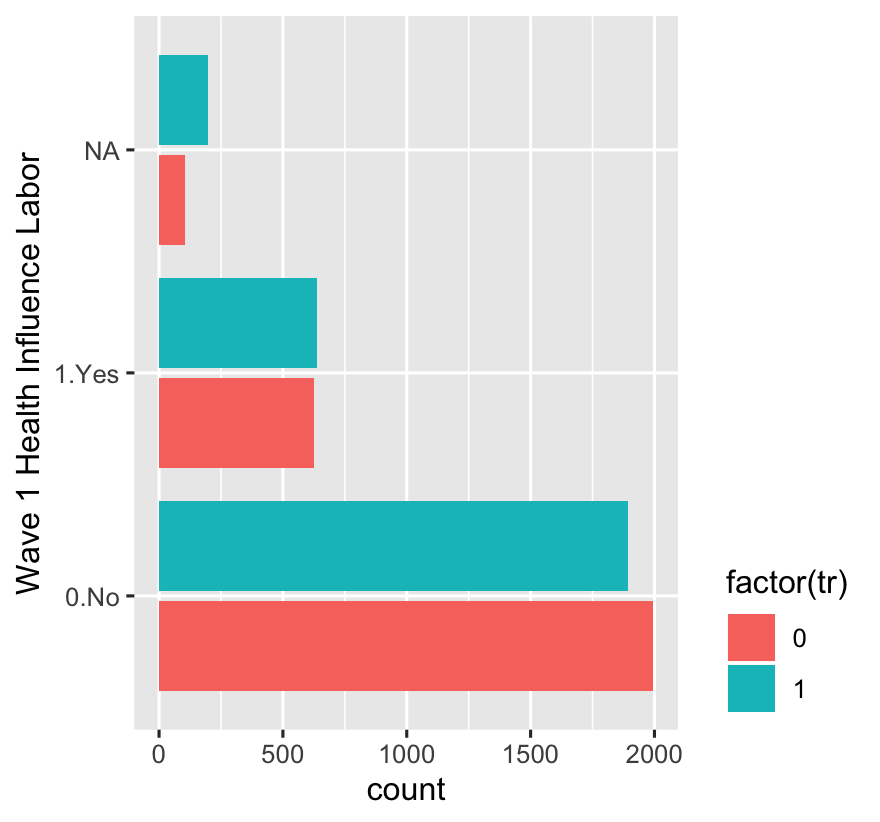
\includegraphics
[width=2.5in]
{W1HealthLabor.png}
\end{figure}
}
\frame
{
\frametitle{Matching results}
\vskip 0.1in  

\begin{figure}[!ht]
\centering
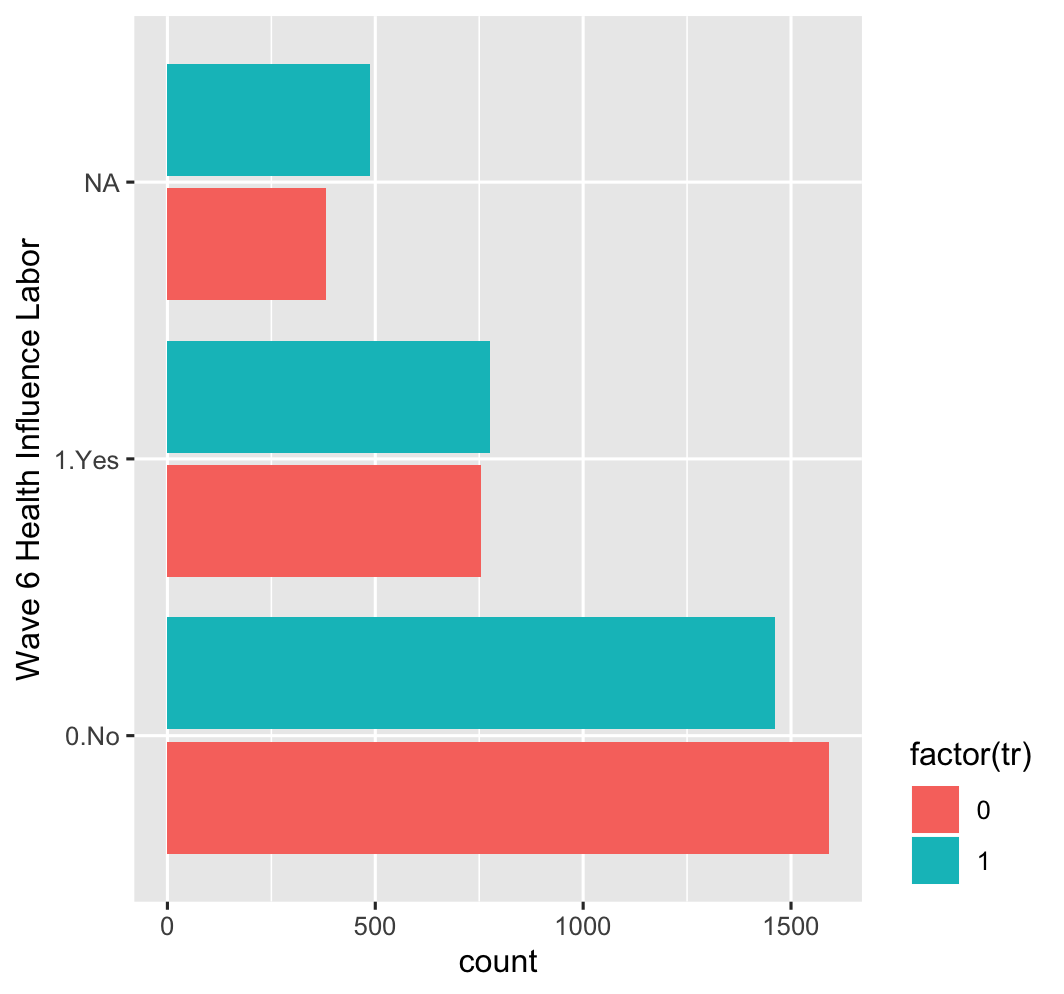
\includegraphics
[width=2.5in]
{W6HealthLabor.png}
\end{figure}
}
\frame
{
\frametitle{Matching results}
\vskip 0.1in  

\begin{figure}[!ht]
\centering
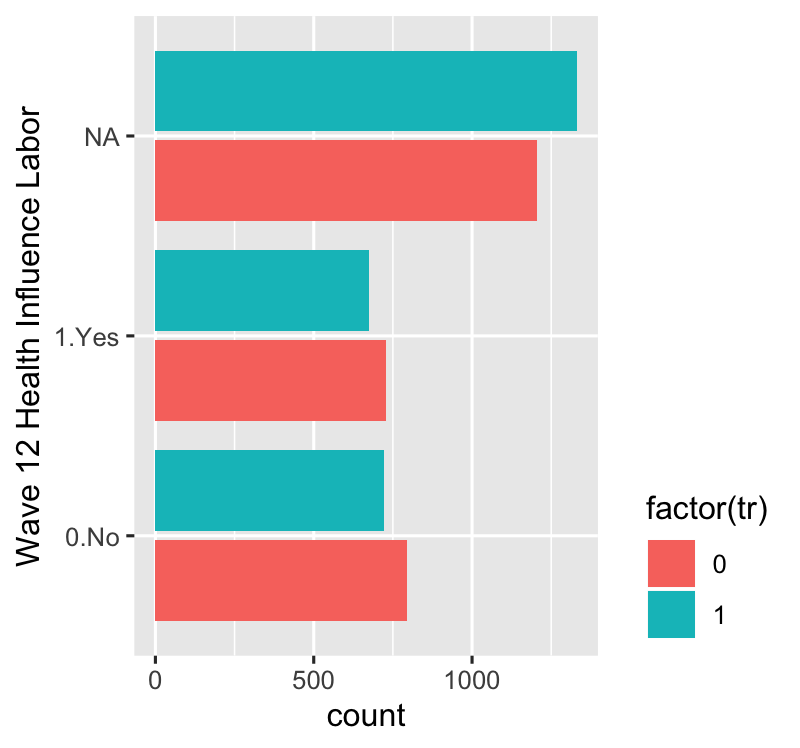
\includegraphics
[width=2.5in]
{W12HealthLabor.png}
\end{figure}
}

\frame
{
\frametitle{Matching results}
\vskip 0.1in  

\begin{figure}[!ht]
\centering
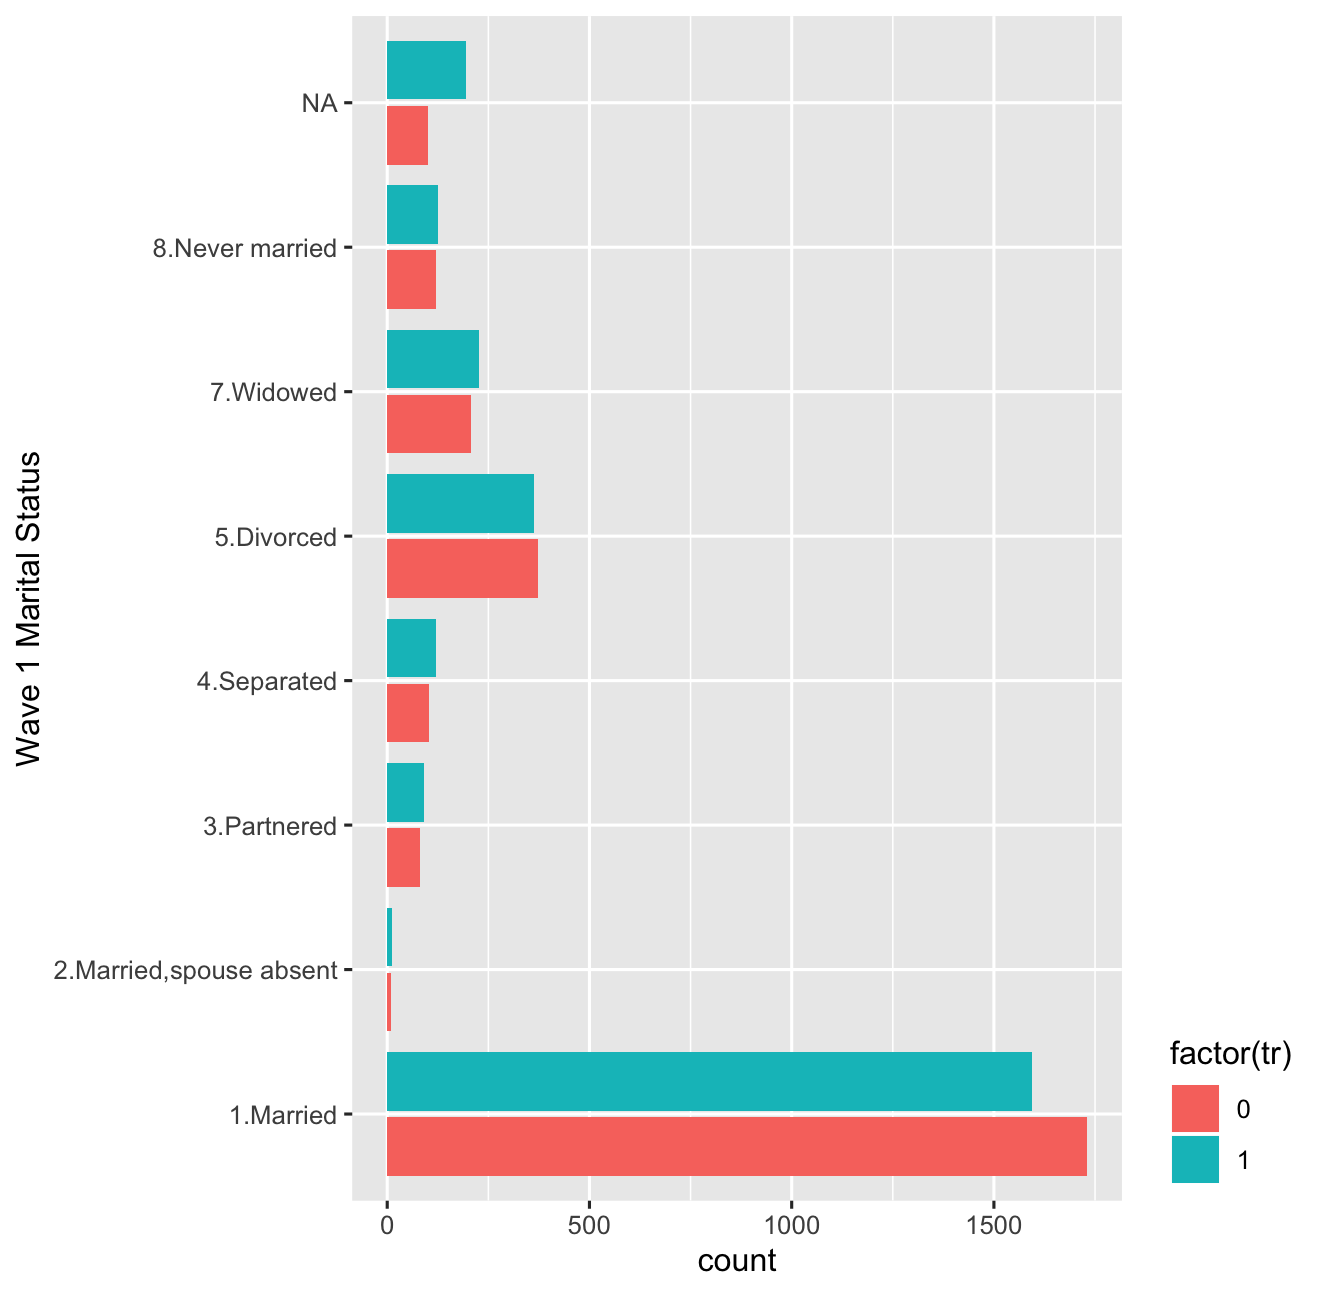
\includegraphics
[width=2.5in]
{W1Marital.png}
\end{figure}
}

\frame
{
\frametitle{Matching results}
\vskip 0.1in  

\begin{figure}[!ht]
\centering
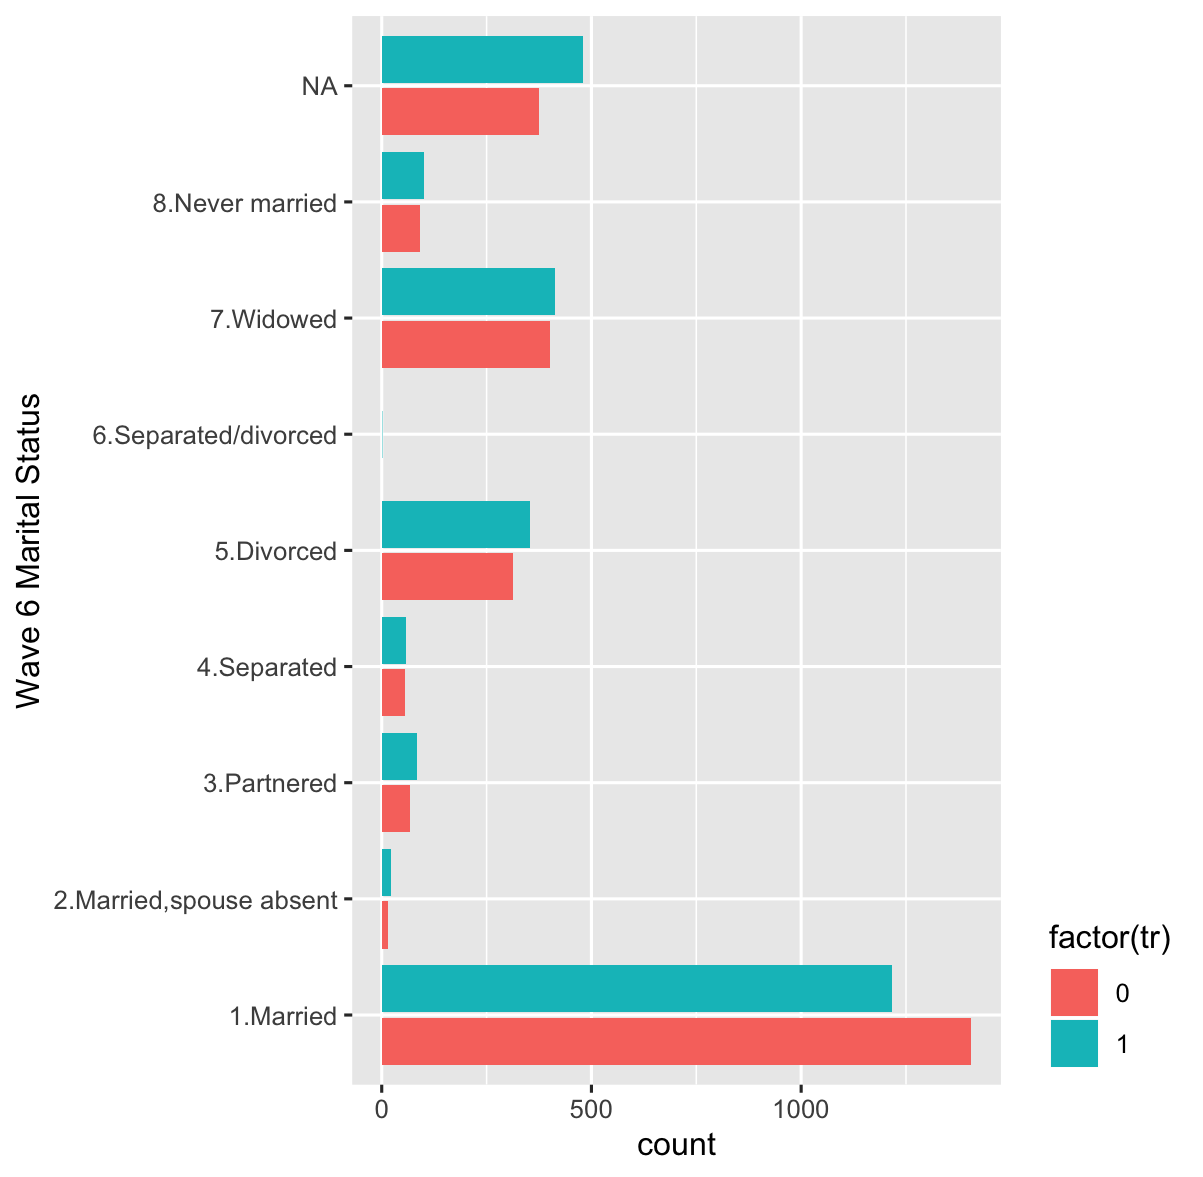
\includegraphics
[width=2.5in]
{W6Marital.png}
\end{figure}
}

\frame
{
\frametitle{Matching results}
\vskip 0.1in  

\begin{figure}[!ht]
\centering
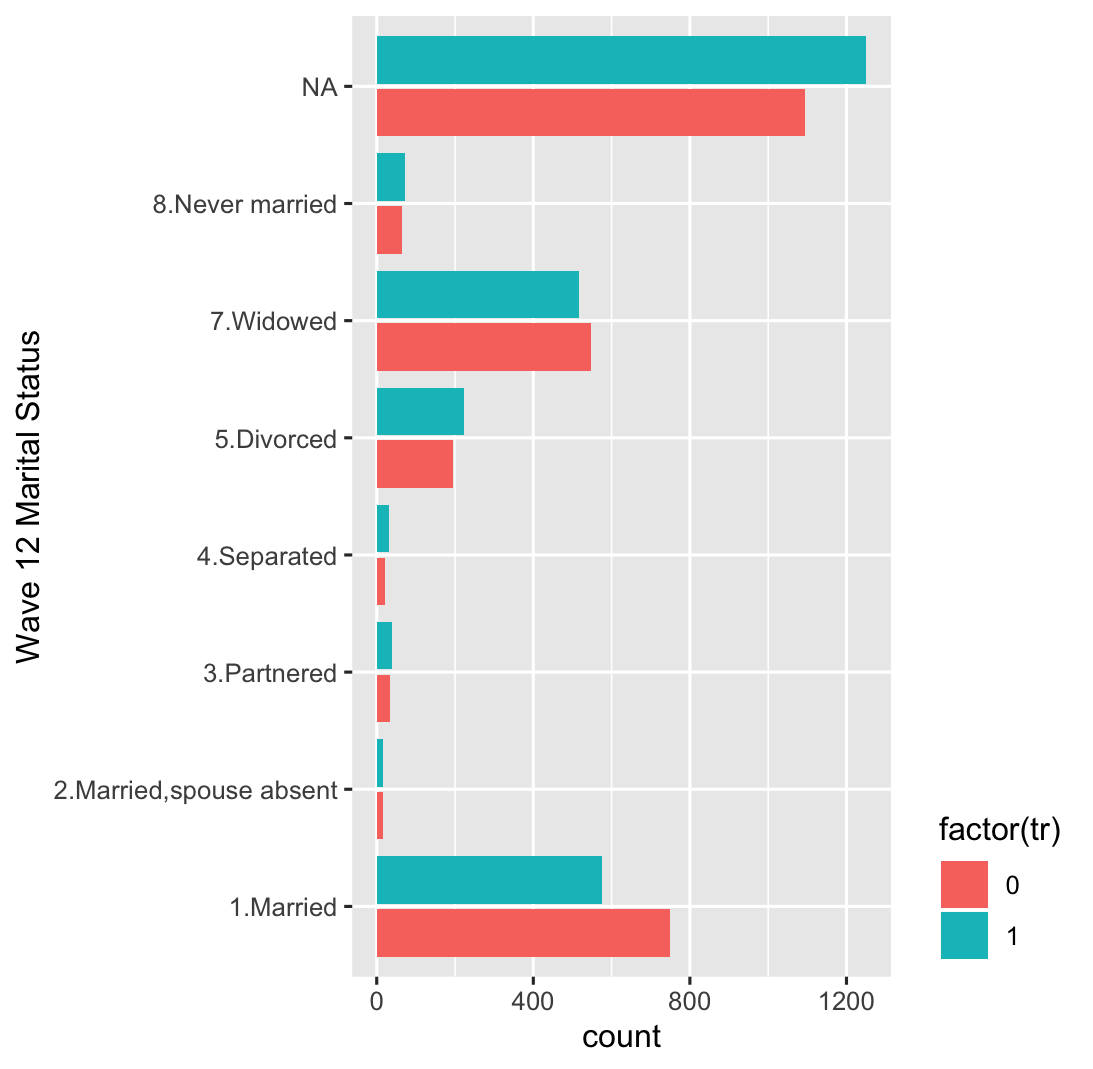
\includegraphics
[width=2.5in]
{W12Marital.png}
\end{figure}
}

\frame
{
\frametitle{Matching results}
\vskip 0.1in  

\begin{figure}[!ht]
\centering
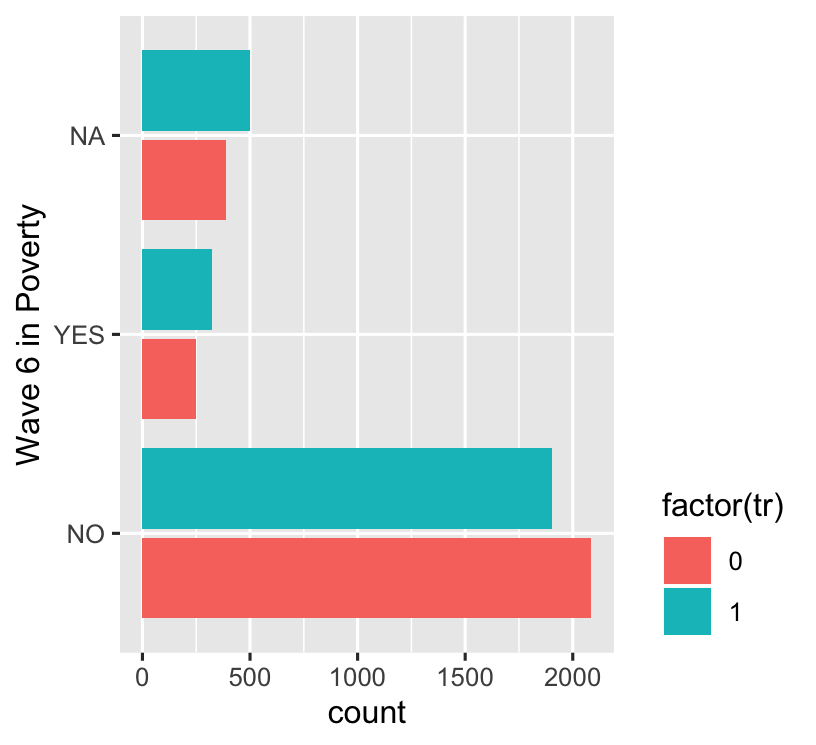
\includegraphics
[width=2.5in]
{W6Pov.png}
\end{figure}
}

\frame
{
\frametitle{Matching results}
\vskip 0.1in  

\begin{figure}[!ht]
\centering
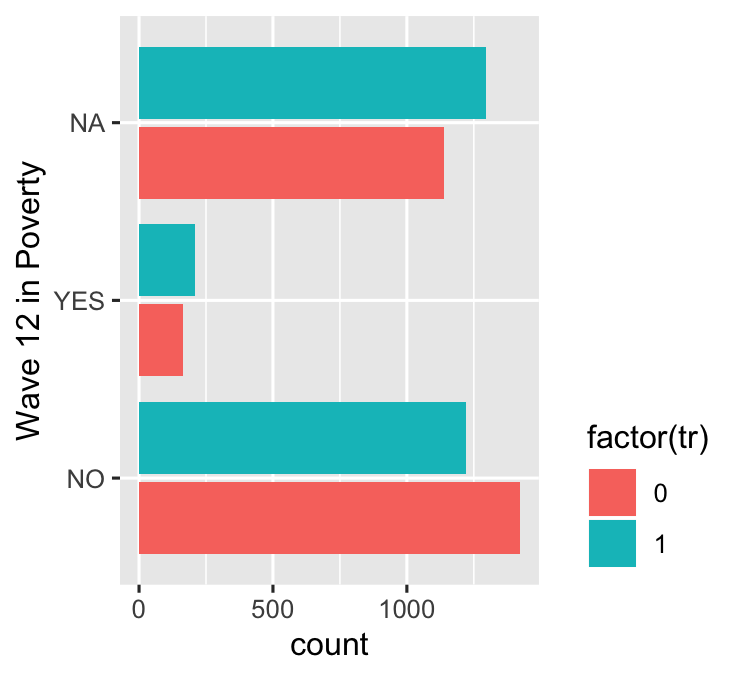
\includegraphics
[width=2.5in]
{W12Pov.png}
\end{figure}
}

\frame
{
\frametitle{Matching results}
\vskip 0.1in  

\begin{figure}[!ht]
\centering
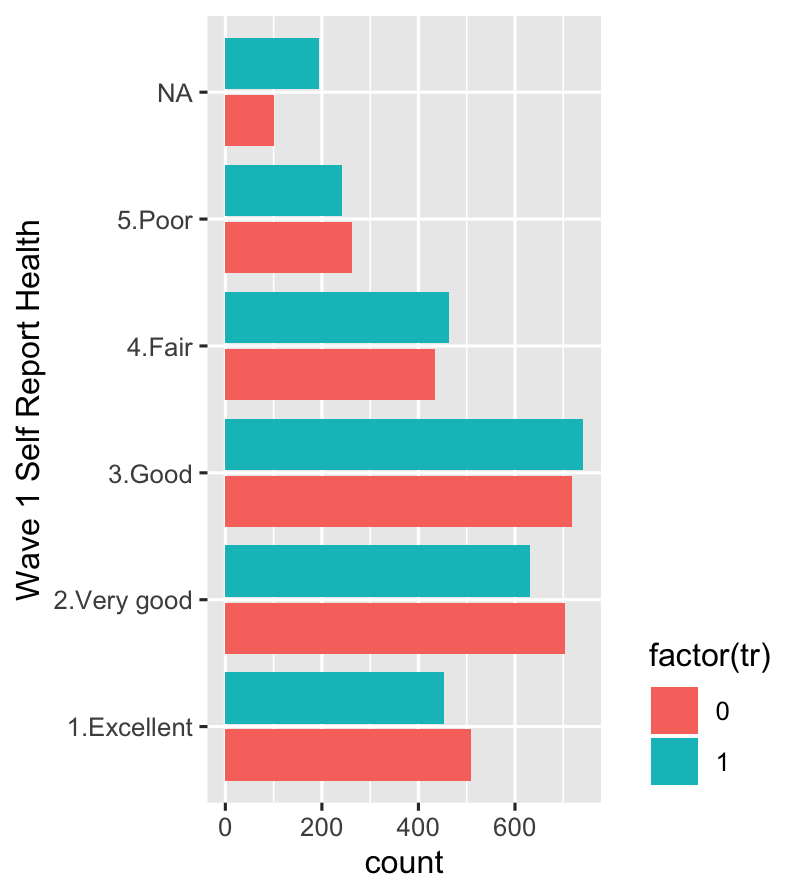
\includegraphics
[width=2.5in]
{W1SelfHealth.png}
\end{figure}
}

\frame
{
\frametitle{Matching results}
\vskip 0.1in  

\begin{figure}[!ht]
\centering
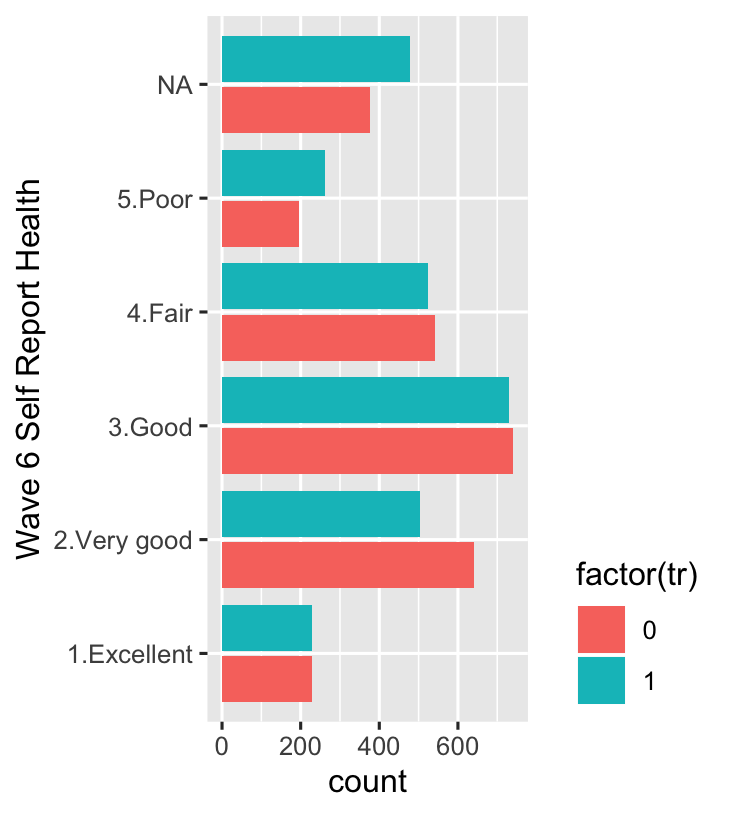
\includegraphics
[width=2.5in]
{W6SelfHealth.png}
\end{figure}
}

\frame
{
\frametitle{Matching results}
\vskip 0.1in  

\begin{figure}[!ht]
\centering
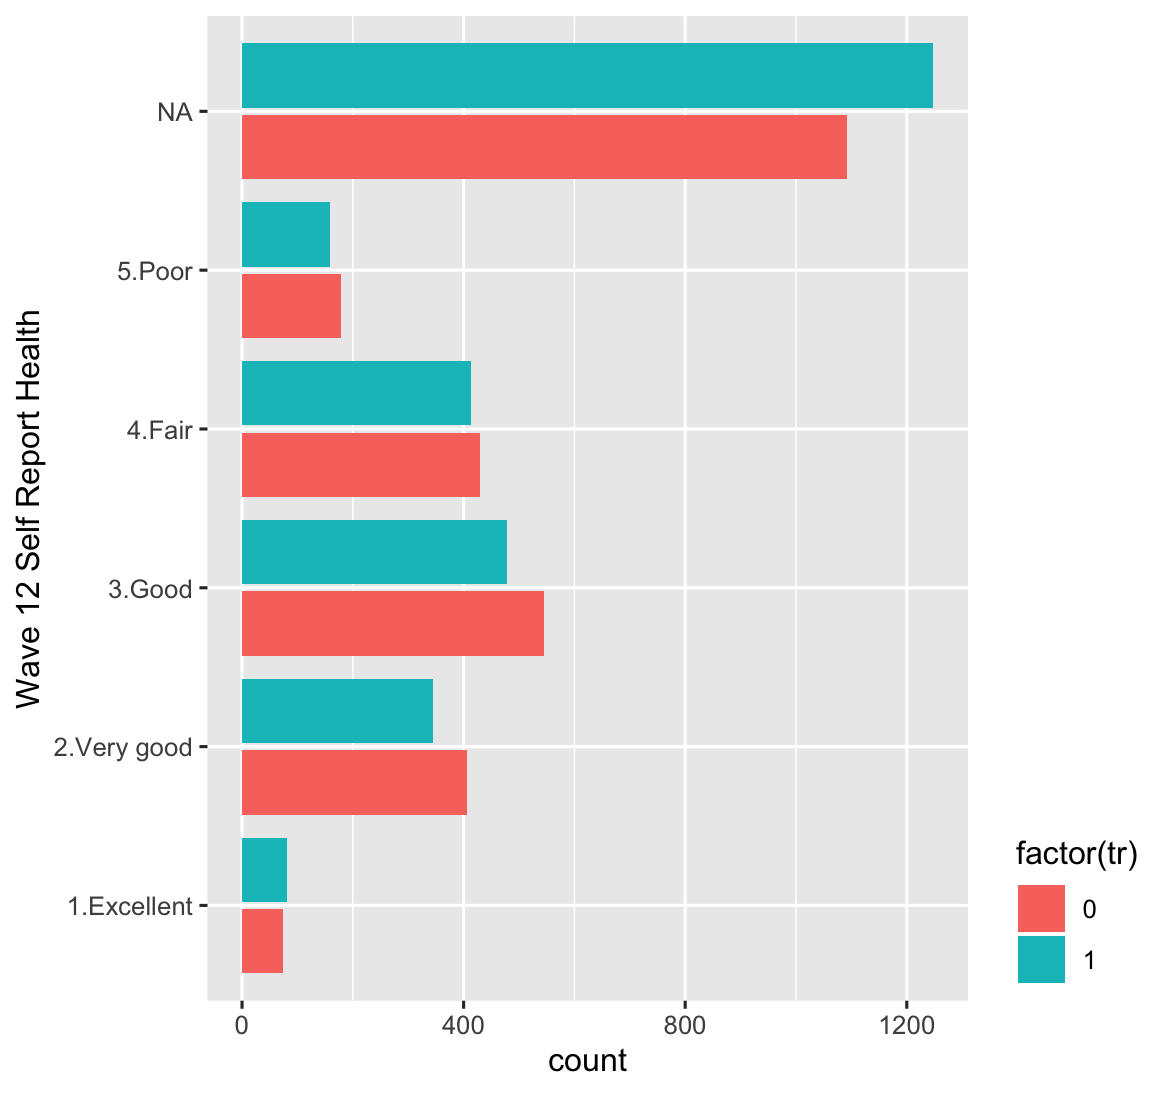
\includegraphics
[width=2.5in]
{W12SelfHealth.png}
\end{figure}
}

\frame
{
\frametitle{Matching results}
\vskip 0.1in  

\begin{itemize}
{
  
\item We obtain 2726 pairs out of 3497 treated individuals. This indicates 771 treated individuals are paired with those who are treated earlier. 

\vskip 0.1in  

\item Death status is recorded for each pair in two subsequential waves. For example, if observation 1 is paired with 2 at wave $t$, and 1 died at wave $t+1$ while 2 died at wave $t+3$, then death status of 1 is "yes" while that of 2 is "no".

\vskip 0.1in  

\item The p-value of pairwise t-test is$ 1.07\times 10^{-7}$, with mean difference 0.031. So the treatment effect is significant.

}
\end{itemize}
}

\frame
{
\frametitle{Sensitivity analysis}
\vskip 0.1in  

\begin{table}[!ht] %[bhtp]
\centering
\caption{\textsl{Summary table overall sensitivity analysis}}
\label{Table-1}
\begin{tabular}{|c|c|}
\hline
$\Gamma$ & p-value \\
\hline
1.0 & 0.000 \\
\hline
1.1 & 0.000 \\
\hline
1.2 & 0.000 \\
\hline
1.3 & 0.001 \\
\hline
1.4 & 0.004 \\
\hline
1.5 & 0.016 \\
\hline
1.59 & 0.045 \\
\hline
1.6 & 0.050 \\
\hline
\end{tabular}
\end{table}
}

\frame
{
\frametitle{Sensitivity analysis}
\vskip 0.1in 

\begin{itemize}
{
  
\item The e-value is 1.59.

\vskip 0.3in  

\item Insensitive to unmeasured confounders.

}
\end{itemize}
}

\frame
{
\frametitle{Heterogeneous Effects}
\vskip 0.1in 

\begin{table}[!ht] %[bhtp]
\centering
\caption{\textsl{ATE among different gender}}
\label{Table-2}
\begin{tabular}{|c|c|}
\hline
Gender & ATE \\
\hline
All & 0.031 \\
\hline
Female & 0.031 \\
\hline
Male & 0.031 \\
\hline
\end{tabular}
\end{table}
}

\frame
{
\frametitle{Heterogeneous Effects}
\vskip 0.1in 

\begin{table}[!ht] %[bhtp]
\centering
\caption{\textsl{ATE among people in different health condition}}
\label{Table-3}
\begin{tabular}{|c|c|}
\hline
Health condition & ATE \\
\hline
All & 0.031 \\
\hline
Excellent & 0.018 \\
\hline
Very good & 0.011 \\
\hline
Good & 0.027 \\
\hline
Fair & 0.025 \\
\hline
Poor & 0.101 \\
\hline
\end{tabular}
\end{table}
}

\frame
{
\frametitle{Heterogeneous Effects}
\vskip 0.1in  

\begin{figure}[!ht]
\centering
\includegraphics
[width=3in, height = 3in]
{ATE.png}
\end{figure}
}

\section*{}
\frame
{
\frametitle{}

\vskip 0.1in

\begin{center}
Thank you!
\end{center}
}





\end{document}